\documentclass[11pt, oneside]{article}   	% use "amsart" instead of "article" for AMSLaTeX format
\usepackage{array}
\setlength{\parindent}{0em}
\setlength{\parskip}{1em}

\usepackage{geometry}                		% See geometry.pdf to learn the layout options. There are lots.
\geometry{letterpaper}                   		% ... or a4paper or a5paper or ... 
%\geometry{landscape}                		% Activate for rotated page geometry
%\usepackage[parfill]{parskip}    		% Activate to begin paragraphs with an empty line rather than an indent
\usepackage{graphicx}				% Use pdf, png, jpg, or eps§ with pdflatex; use eps in DVI mode
								% TeX will automatically convert eps --> pdf in pdflatex		
\usepackage{amssymb}
\usepackage{listings}
\usepackage{tikz-qtree}

%SetFonts

%SetFonts


\title{COMP9417 - Assignment 2}
\author{Avinash K. Gupta, Yuyang Shu, Maria Oei}
%\date{}							% Activate to display a given date or no date

\begin{document}
\maketitle


\section{Introduction}

With over 100 millions of monthly visitor in Quora, it is inevitable that many people are asking similar questions. This has become an issue as user has to read through responses to many questions in order to find the best answer. The aim of this project is to implement algorithms to identify 2 similar questions which can help Quora in improving user experience by finding high quality answers to questions.

The 2 approaches used in this project were perceptron learning and LSTM. In the perceptron learning, we used 3 inputs which measured semantic similarity, word order and word overlaps between 2 sentences.

In LSTM, bla bla bla bla

We will see that for our case the performance of the 2 models were quite similar. However, there are other research done on LSTM where it has been shown that LSTM has the potential to performs well with enough training and with careful selection of initial weight.
%\subsection{}

\section{Methodology}

\subsection{Perceptron Learning}
- What do we implement (Theory)
- How do we implement it


\subsection{LSTM - RNN}
\subsubsection{Overview}
\par In this approach, we present  siamese adaption of Long Short-Term Memory(LSTM) network for labeled data contains pairs of variable-length sequences. This model is used to get the semantic similairty between the sentences using complex neural network. For this applications, we provide word-embedding vectors supplemented with synonymic information to the LSTMs, which use a fixed size vector to convert the syntactic meaning of the sentence. 

\subsubsection{Model}
\par It's a supervised learning model, where each data consists of pair of sequences 
$(x_1^{(a)},...,x_{n_a}^{(a)})$, $(x_1^{(b)},...,x_{n_b}^{(b)})$ of fixed size vectors along with a single label y(human labeled) for the pair. Note that sequences may be differenent length. These data will be pass to the model with a purpose of learning the semantics. 
 \begin{figure}[h]
    \centering
    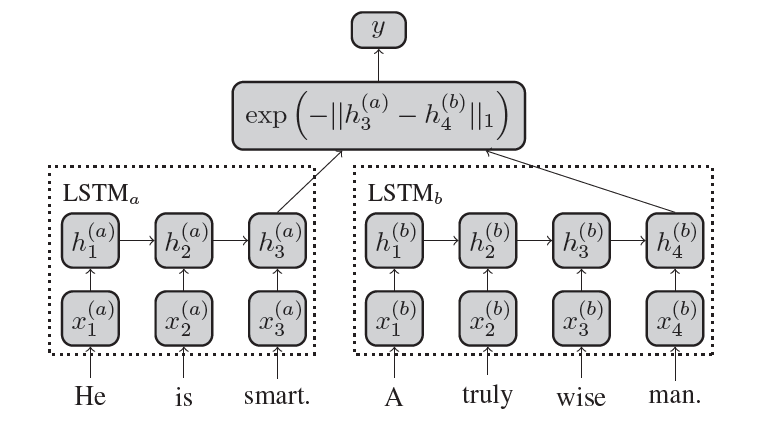
\includegraphics[width=.75\textwidth]{lstm_image}
    \caption{lstm architecture}
\end{figure}
In the above diagram, there are two networks $LSTM_a$ and $LSTM_b$, each of them process a sentence in a given pair and predict whether  $LSTM_a=LSTM_b$ based on the similarity between the vectors. In each LSTM, the word vector is employ to the hidden layer and calculation is done and output is passed to the next hidden layer to remember the previous context and so on.
 \begin{figure}[h]
    \centering
    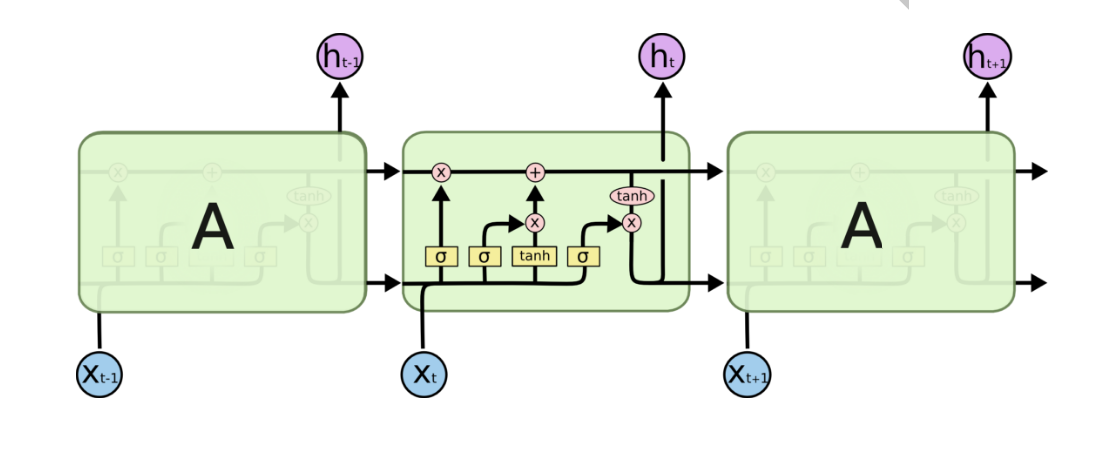
\includegraphics[width=.85\textwidth]{hidden_layer}
    \caption{repeating module of hidden layer}
\end{figure}
In above figure, the hidden layer which is core part of our neural network. It performs operation listed below on each word vector.
\begin{itemize}
\item The first sigmoid function is used to decide which information to keep and what to ignore
$$f_t=sigmoid(W_ix_t + U_ih_{t-1}+b_i)$$
\item Now it's time to update the old cell state into new cell state. The last step already decided what to do, in this step we just actually need to do it.
$$i_t=sigmoid(W_fx_t + U_fh_{t-1}+b_f)$$
$$c_t^`=\tanh(W_cx_t + U_ch_{t-1}+b_c)$$
\item In this step, we will multiply old state $c_{t-1}$ with $f_t$ to forget things we decided to forget earlier. Then we add to new candidate values
$$c_t=i_t \odot c_t^` + f_t \odot c_{t-1}$$
\item Final step defines what we actually need to output based on out filtered cell state and then $\tanh$(used to push values between -1 and 1) and multiply with sigmoid function to decide the parts we need to output.
$$o_t=sigmoid(W_ox_t + U_oh_{t-1}+b_o)$$
$$h_t=o_t \odot \tanh(c_t)$$
\end{itemize}

Above process are carried by both the LSTM and emploed to the Similarity Function given below, which calculates the Manhattan differnece between the ouputs.
$$g(h_{T_a}^{(a)},h_{T_b}^{(b)})=\exp(\textendash \parallel h_{T_a}^{(a)} \textendash h_{T_b}^{(b)}\parallel_1) \in [0,1]. $$
\subsection{LSTM - RNN}
\subsubsection{Overview}
\par In this approach, we present  siamese adaption of Long Short-Term Memory(LSTM) network for labeled data contains pairs of variable-length sequences. This model is used to get the semantic similairty between the sentences using complex neural network. For this applications, we provide word-embedding vectors supplemented with synonymic information to the LSTMs, which use a fixed size vector to convert the syntactic meaning of the sentence. 

\subsubsection{Model}
\par It's a supervised learning model, where each data consists of pair of sequences 
$(x_1^{(a)},...,x_{n_a}^{(a)})$, $(x_1^{(b)},...,x_{n_b}^{(b)})$ of fixed size vectors along with a single label y(human labeled) for the pair. Note that sequences may be differenent length. These data will be pass to the model with a purpose of learning the semantics. 
 \begin{figure}[h]
    \centering
    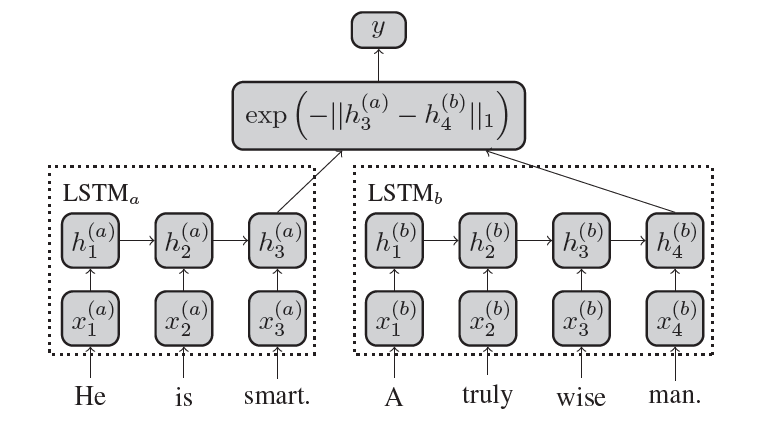
\includegraphics[width=.75\textwidth]{lstm_image}
    \caption{lstm architecture}
\end{figure}
In the above diagram, there are two networks $LSTM_a$ and $LSTM_b$, each of them process a sentence in a given pair and predict whether  $LSTM_a=LSTM_b$ based on the similarity between the vectors. In each LSTM, the word vector is employ to the hidden layer and calculation is done and output is passed to the next hidden layer to remember the previous context and so on.
 \begin{figure}[h]
    \centering
    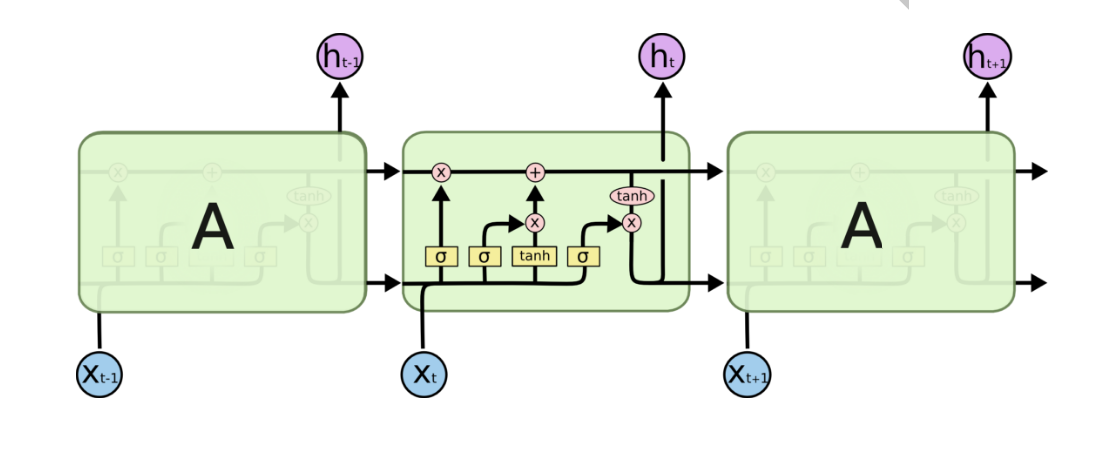
\includegraphics[width=.85\textwidth]{hidden_layer}
    \caption{repeating module of hidden layer}
\end{figure}
In above figure, the hidden layer which is core part of our neural network. It performs operation listed below on each word vector.
\begin{itemize}
\item The first sigmoid function is used to decide which information to keep and what to ignore
$$f_t=sigmoid(W_ix_t + U_ih_{t-1}+b_i)$$
\item Now it's time to update the old cell state into new cell state. The last step already decided what to do, in this step we just actually need to do it.
$$i_t=sigmoid(W_fx_t + U_fh_{t-1}+b_f)$$
$$c_t^`=\tanh(W_cx_t + U_ch_{t-1}+b_c)$$
\item In this step, we will multiply old state $c_{t-1}$ with $f_t$ to forget things we decided to forget earlier. Then we add to new candidate values
$$c_t=i_t \odot c_t^` + f_t \odot c_{t-1}$$
\item Final step defines what we actually need to output based on out filtered cell state and then $\tanh$(used to push values between -1 and 1) and multiply with sigmoid function to decide the parts we need to output.
$$o_t=sigmoid(W_ox_t + U_oh_{t-1}+b_o)$$
$$h_t=o_t \odot \tanh(c_t)$$
\end{itemize}

Above process are carried by both the LSTM and emploed to the Similarity Function given below, which calculates the Manhattan differnece between the ouputs.
$$g(h_{T_a}^{(a)},h_{T_b}^{(b)})=\exp(\textendash \parallel h_{T_a}^{(a)} \textendash h_{T_b}^{(b)}\parallel_1) \in [0,1]. $$
\section{Result}
How do they perform

\section{Discussion}
\subsection{Conclusion}
 \subsection{Limitation \& Improvement}



\end{document}  